\documentclass[a4paper,12pt]{report}
\usepackage[utf8]{inputenc}
\usepackage[T1]{fontenc}
\usepackage[ngerman]{babel}
\usepackage[parfill]{parskip}
%\usepackage{eurosans}
\usepackage[top=3cm, left=3cm]{geometry}
\usepackage{setspace}
\usepackage{mdwlist}
\usepackage{graphicx}
\usepackage{eurosym}
\renewcommand*\familydefault{\sfdefault}

\setcounter{secnumdepth}{-1}

\begin{document}

\title{\textbf{ESE-Stadtführungsführer 2015}\\}
\date{}
\author{mit Inhalten von\\Adrian Ackermann, Anna Brauer, Martin Eisoldt,\\Sara Groß, Philipp Heisig, Ulrich Huber,\\ Matthias Lehne, Franz-Wilhelm Schumann}
\maketitle

\chapter{Hinweise für Tutoren}
\section{Ansprechpartner}
Franz (franz@ifsr.de): 0152/55477616\\
FSR/ESE-Orga (ese-orga@ifsr.de): 0351/463-38226


\section{Über die Stadtführung}
\begin{itemize*}
\item Ziel der Stadtführung ist Vermittlung von Informationen rund um die Sehenswürdigkeiten in Dresden.
\item Der Inhalt dieser Handreichung ist keine strike Vorgabe, ihr könnt Infomationen weglassen oder weitere hinzufügen.
Richtet euch bei bei der Führung nach der Stimmung der Erstsemester.
Ihr könnt die Stichpunkte gerne noch mit eigenen Einfällen ergänzen.
\item Versucht die Stadtführung interessant zu gestalten. Lest nicht nur stur die Informationen und Jahreszahlen ab sondern versucht auch teilweise lustige Sidefacts zu bieten.
\end{itemize*}

\section{Vor der Stadtführung zu erledigende Dinge}
\begin{itemize*}
\item Lest euch die Informationen schon mal im Ganzen durch.
Es wäre schlecht, wenn ihr das erst bei der Stadtführung selbst tun müsst!
Markiert euch eventuell wichtige Punkte.
Wenn ihr Fragen habt, stellt diese dem leitendem Tutor.
\item Seid im Vorfeld mit der Route vertraut. Gegebenenfalls macht eine Proberunde.
\item Sucht euch passende Orte an den Stationen aus, wo ihr mit den Erstsemestern stehen bleiben könnt (keine Gefährdung durch Verkehr, etwas ruhiger damit man euch versteht, mit gutem Blick auf die Sehenswürdigkeit).
\end{itemize*}

\newpage

\section{Die Tour}
\begin{itemize*}
\item Startpunkt ist der freie Platz vor der Altmarkt-Galerie in der Nähe der Haltestelle Prager Straße (51.047517, 13.736457)
\item Es gibt folgende Stationen: (Tour-Reihenfolge)\\Altmarkt, Residenzschloss, Cholerabrunnen, Zwinger, Semperoper / Theaterplatz, Kathedrale (Hofkirche), Fürstenzug, Frauenkirche, Festung Dresden, Brühlsche Terassen, Augustusbrücke, Japanisches Palais, Goldener Reiter\\
\end{itemize*}
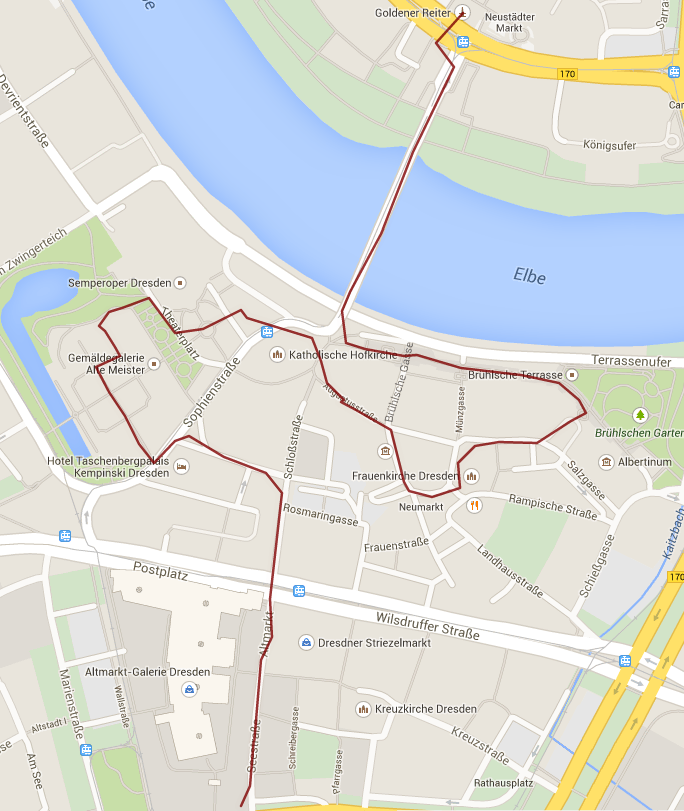
\includegraphics[width=\linewidth]{./tour.png}

\chapter{Zu vermittelnde Informationen}

\section{1. Altmarkt}
\begin{itemize*}
\item ältester Platz Dresdens, hat den Namen seit fast 500 Jahren nach Entstehung des Neumarkts
\item schon immer umgeben von Wohn- und Geschäftshäusern und wichtigen Straßen
\item hier wurden nach dem Bombenagriff am 13. Februar 1945 fast 7.000 Leichen verbrannt
\item Platz für diverse Veranstaltungen über das Jahr hinweg (z.B. Striezelmarkt, einer der ältesten deutschen Weihnachtsmärkte)
    \begin{itemize*}
    \item Größte Kirche Sachsen (über 3.000 Plätze)
    \item Mehrmals zerstört und immer wieder aufgebaut (zuletzt im 2. Weltkrieg)
    \end{itemize*}
\item Im Norden: Kulturpalast
    \begin{itemize*}
    \item Mehrzwecksaal der 1969 eingeweiht wurde
    \item Wird zurzeit umgebaut um eine bessere Akkustik zu gewährleisten
    \item An der Seite: Wandbild „Weg der roten Fahne“, mittlerweile Kulturdenkmal
    \end{itemize*}
\end{itemize*}

\section{2. Residenzschloss}
\begin{itemize*}
\item war das Residenzschloss der sächsischen Kurfürsten (1547–1806) und Könige (1806–1918)
\item eines der ältesten Bauwerke der Stadt und baugeschichtlich bedeutsam, da alle Stilrichtungen von Romanik bis Historismus vertreten sind
\item brannte im 2. WK bis auf Grundmauern nieder, Wiederaufbau ab 1985
    \begin{itemize*}
    \item 1991 bekam der Hausmannsturm seine Spitze zurück
    \item 2004 Einrichtung der Kunstbibliothek, des Kupferstichkabinetts und des Neuen Grünen Gewölbes
    \item 2006 Historisches Grünes Gewölbe
    \item 2010 Türckische Kammer
    \end{itemize*}
\item beherbergt heute fünf Museen:
    \begin{itemize*}
    \item Historisches und Neues Grünes Gewölbe
    \item Münzkabinett
    \item Kupferstichkabinett
    \item Rüstkammer Türckische Kammer
    \end{itemize*}
\end{itemize*}
\subsection{Sidefacts Residenzschloss}
\begin{itemize*}
\item nach dem 2. WK wurde in einem Teil der Kellergewölbe einige Jahre lang eine Pilzzucht betrieben
\item in den ersten Jahren nach Wiedereröffnung des Hist. Gr. Gewölbe musste man Tickets lange im Voraus kaufen (bis zu einem Jahr)
\item bei Caterings im Innenhof ist der Ausschank von Rotwein (meistens) verboten, wegen des Sandsteinbodens
\end{itemize*}

\section{3. Cholerabrunnen}
\begin{itemize*}
\item auch Gutschmid-Brunnen, von Freiherr Eugen von Gutschmid finanziert
\item sollte Dank ausdrücken, dass Dresden Mitte des 19. Jahrh. von der Cholera verschont wurde
\end{itemize*}

\section{4. Zwinger}
\begin{itemize*}
\item 1709-1732 von bedeutendem Architekten Pöppelmann erbaut
\item im Auftrag von August dem Starken, der die Künste und das Vergnügen jeglicher Art liebte und gern wie Ludwig XIV sein wollte, aber weder ein großer Kriegsherr noch ein großer Politiker war, und auch nicht besonders gut mit Geld umgehen konnte
\item als Festplatz für die Hofgesellschaft gedacht, außerdem als Orangerie für die Orangenbäume
\item der Name „Zwinger“ kommt daher, da der Raum zwischen der äußeren und der inneren Festungsmauer als Zwinger bezeichnet wurde
\item August III war noch vernarrter in die Kunst als sein Vater, sodass er mit dem Architekten Gottfried Semper die vierte Seite des Zwingers als Gemäldegalerie bauen ließ (die „Alten Meister“)
\item Zwinger beherbergt neben Gemäldegalerie noch die kurfürstliche Porzellansammlung und den mathematisch-physikalischen Salon
\item das „Nymphenbad“, ein barocker Brunnen (verlassen des Zwingers durch das Nymphenbad)
\item jede Viertelstunde kann man das Porzellanglockenspiel hören
\end{itemize*}

\section{5. Semperoper / Theaterplatz}
\begin{itemize*}
\item ist das Opernhaus der Sächsischen Staatsoper Dresden
\item die Dresdner Phillharmoniker gelten als eines der besten Orchester der Welt
\item nach ihrem Architekten Gottfried Semper benannt
\item 1871-1878 erbaut (nachdem 1869 das vorherige Theaterhaus abgebrannt ist)
\item nach Entwurf von G. Semper, aber unter Leitung seines Sohnes gebaut (er war im Exil)
\item im 2. WK komplett zerstört - ab 1977 Wiederaufbau
\item am 13. Februar 1985 (40. Jahrestag der kriegsbedingten Zerstörung) konnte die Semperoper mit Carl Maria von Webers Oper Der Freischütz wiedereröffnet werden (mit dieses Werk wurde das Opernhaus am 31. August 1944 geschlossen)
\item auf/an Theaterplatz:
    \begin{itemize*}
    \item bronzene Reiterstandbild des sächsischen Königs Johann (1889 geschaffen)
    \item Brunnen und Carl-Maria-von-Weber-Denkmal
    \item Italienisches Dörfchen
    \end{itemize*}
\end{itemize*}
\subsection{Sidefacts Semperoper / Theaterplatz}
\begin{itemize*}
\item weil die Semperoper in der Radeberger Bier Werbung zu sehen ist, denken viele es wäre die Brauerei
\item in der Zeit des Nationalsozialismus hieß der Theaterplatz Adolf-Hitler-Platz
\end{itemize*}

\section{6. Kathedrale (Hofkirche)}
\begin{itemize*}
\item ist Kathedrale des Bistums Dresden-Meißen (seit 1980) sowie eine Stadtpfarrkirche Dresdens
\item unter Kurfürst Friedrich August II. von Sachsen (durch Gaetano Chiaveri) von 1739 bis 1755 im Stil des Barocks errichtet
\item ist durch einen Übergang mit dem Residenzschloss verbunden
\item wurde im 2. WK stark zerstört, aber schon ab Juni 1945 wieder für Messen genutzt (Bennokapelle, dann linker Seitenflügel) ab 1962 konnte sie wieder komplett genutzt werden
\end{itemize*}
\subsection{Sidefacts Kathedrale}
\begin{itemize*}
\item Hauptgrund für Bau: Sachsen war zwar evangelisch, aber eine katholische Kirche wurde in Dresden benötigt, weil August der Starke König von Polen werden wollte (musste als König ebenfalls katholisch werden)
\item in Grabgewölben wurden viele Wettiner Könige + Familie beigesetzt, das Herz August des Starken befindet sich hier in einer Kapsel in der Stiftergruft
\end{itemize*}

\section{7. Fürstenzug}
\begin{itemize*}
\item besteht aus ca. 23000 Fliesen aus Meißner Porzellan
\item 102 Meter lang
\item zeigt Ahnengalerie von 1127 bis 1904 - Grafen, Herzoge, Kurfürsten und Könige
\item während des 2. WK nur mininmal zerstört, da das Porzellan den hohen Temperaturen standhalten konnte
\end{itemize*}

\section{8. Frauenkirche}
\begin{itemize*}
\item das bekannteste Wahrzeichen der Stadt
\item wurde im 2. Weltkrieg zerstört, aber nicht durch Bomben
    \begin{itemize*}
    \item diese prallten von der Kuppel ab, aber die hohen Temperaturen durch den Feuersturm machten den Sandstein spröde, so dass sie 2 Tage später zusammenbrach
    \item Zerstörung war für Dresdner von hoher Symbolkraft, da damit auch der letzte Teil des alten Dresdens zerstört war
    \end{itemize*}
\item in der DDR diente die Ruine als Mahnmal gegen den Krieg
\item 2005 wurde der ausschließlich durch Spenden finanzierte Wiederaufbau beendet
\item einzigartig auf der Welt: die am unteren Ende nach innen gewölbte Kuppel - ähnlich einer Glocke
\item schwarze Steine sind Steine der alten Kirche (insgesamt 43\% der Kirche), allerdings keine in Kuppel wiederverwendet, da hohe Stabilität enorm wichtig ist
\item das Kreuz wurde von Sohn eines britischen Bomberpilots gefertigt, der auch die Angriffe auf Dresden flog
\end{itemize*}

\section{9. Festung Dresden}
\begin{itemize*}
\item 1299 erstmals erwähnt
\item umfasste Innere Altstadt (Prager Straße) bis Innere Neustadt (Albertplatz bzw. 300m nördlich vom goldenen Reiter)
\item es gab fünf Stadttore, meherere Bastionstürme und Mauertürme
\item entfestigt und zurückgebaut bis 1811, heute sind kaum noch Befestigungsanlagen zu erkennen
\item seit 1992 Museum im erhaltenen Teil der Dresdner Befestigungsanlagen
\end{itemize*}

\section{10. Brühlsche Terassen und Umgebung}
\begin{itemize*}
\item der „Balkon Europas“ genannt - wegen des schönen Ausblicks auf die Elbe und der Tatsache, dass sich viele historisch wichtige Gebäude an ihr entlang aufreihen, zb das Albertinum, das Johanneum und die Kunstakademie (auch als „Zitronenpresse“ bezeichnet)
\item Graf Brühl machte den Festungswall im 18. Jh zu seinem privaten Lustgarten
\item Elbwiesen mit Filmnächten (Konzerte und Filme im Sommer)
\item Sächsische Dampfschifffahrt
    \begin{itemize*}
    \item älteste/größte Raddampferflotte der Welt
    \item 9 Raddampfer, 7 davon aus den Jahren 1879-1898
    \item Linienfahrten bis Bad Schandau, Tourismusfahrten
    \end{itemize*}
\item zwei „Jahrhunderthochwasser“ (2002 und 2013) der Elbe mit vielen Schäden in ganz Dresden und Umgebung
\end{itemize*}

\section{11. Augustusbrücke}
\begin{itemize*}
\item erste und älteste Steinbrücke über die Elbe, löst 1275 eine Holzkonstruktion ab und gehört dann mit den damals 25 Bögen zu den längsten Brücken in ganz Deutschland
\item 1729 war es August der Starke, der eine Erweiterung der Brücke vornehmen ließ (wiederum von Pöppelmann), da der zunehmende Verkehr zu viel für die Brücke wurde - erbaute eine der prächtigsten und schönsten Brücken in ganz Europa nach dem Vorbild der Karlsbrücke in Prag
\item kompletter Neubau 1907, da sie für die Straßenbahnen zu eng und für die Schiffe zu niedrig wurde, jedoch nahm man wieder Sandstein und orientierte sich an Pöppelmanns Entwürfen
\item gegen Ende es zweiten Weltkriegs - völlig sinnlos - zu Teilen gesprengt und danach wieder errichtet
\item noch fahren Autos darüber, was in ein paar Jahren aber nicht mehr so sein wird: wenn 2016 die Albertbrücke wieder befahrbar ist, soll die Augustusbrücke für immer kraftfahrzeugfreie Zone werden
\end{itemize*}

\section{12. Japanisches Palais}
\begin{itemize*}
\item Museum für Völkerkunde und Naturhistorische Sammlungen
\item Highlight: Damaskuszimmer - prunkvoll verzierter Empfangsraum eines Damaszener Wohnhauses
\item früher Kurfürstliche Bibliothek, woraus später hauptsächlich die Sächsische Landesbibliothek hervorging
\item 1715 von Rudolph Faesch für Jakob Heinrich Graf von Flemming errichtet (kleineres Landhaus -nicht mehr erkennbar)
\item August der Starke hegte großes Interesse an dem Palais
\item 1727 bis 1733 Umbau in heutige Form (fast komplett) - Name dort erhalten
\item Zerstörungen im im 7jährigen Krieg und 2. WK
\end{itemize*}

\section{13. Goldener Reiter}
\begin{itemize*}
\item 1736 wurde das Denkmal enthüllt (3 Jahre nach dem Tod von August dem Starken)
\item ehemals feuervergoldet, später mit Blattgold restauriert
\item (evtl. Informationen zur Neustadt geben als Abschluss)
\end{itemize*}

\chapter{English content}

\section{1. Altmarkt}
\begin{itemize*}
\item oldest market square in Dresden, called „Altmarkt“ since the building of the „Neumarkt“ 500 years ago
\item surrounded by residential and commercial buildings
\item various events take place at this square through the hole year (e.g. „Striezelmarkt“, one of the oldest christmas markets in germany)
    \begin{itemize*}
    \item largest church in saxony (over 3.000 seats) „Kreuzkirche“
    \item destroyed several times but always rebuilt
    \end{itemize*}
\item „Kulturpalast“
    \begin{itemize*}
    \item event location for concerts etc., first opened in 1969
    \item currently under reconstruction to achieve  better acoustics
    \item on the side: mural „Weg der roten Fahne“, cultural monument
    \end{itemize*}
\end{itemize*}

\section{2. Residenzschloss}
\begin{itemize*}
\item residence of the electors of saxony and the saxon kings between 1547 and 1918
\item one of the oldest and most significant buildings in Dresden, all architectual styles from romanesque to historism are represented
\item burned down during WW2, rebuilding started in 1985
\item toady 5 museums are located inside the building:
    \begin{itemize*}
    \item the historical and the new „Grünes Gewölbe“
    \item Münzkabinett („coin cabinet“)
    \item Kupferstichhkabinett („copper engraving“)
    \item Rüstkammer Türkische Kammer („armory turkish chamber“)
    \end{itemize*}
\end{itemize*}
\subsection{Sidefacts Residenzschloss}
\begin{itemize*}
\item after WW2 a fungus culture was located in some parts of the basement, atleast for several years
\item after the reopening of the historical „Grünes Gewölbe“ in 2006 the visitors had to buy their tickets one year in advance because of very high interest
\item during events inside the courtyard it is (mostly) not allowed to serve red wine because of the white freestone floor
\end{itemize*}


\section{3. Cholerabrunnen}
\begin{itemize*}
\item also called Gutschmid-Spring, baron Eugen von Gutschmid paid for it
\item built in thanks that Dresden was spared by the cholera epidemics in the 19th century
\end{itemize*}

\section{4. Zwinger}
\begin{itemize*}
\item built during 1709-1732 by famous architect Pöppelmann
\item commissioned by August the Strong, a lover of art and pleasure, who strove to be like Louis XIV, despite not being a proficient combat leader or politician, and, on top of that, not being good with money
\item meant to be a place for festivals of the court and as a orangery for the orange trees
\item „Zwinger“ refers to defensive fortification: space between inner and outer castle wall
\item August III loved Art even more than his father so he let Gottfried Semper build the fourth side as an art gallery (today it’s home of the “Gemäldegalerie Alte Meister”)
\item there are as well the electoral porcelain collection and „Mathematisch-Physischer Salon“ (Royal cabinet of Mathematical and Phyiscal Instruments)
„Nymphenbad“, a baroque fountain \textit{(verlassen des Zwingers durch das Nymphenbad)}
\item one can hear the porcelain bells chime every 15 minutes
\end{itemize*}

\section{5. Semperoper / Theaterplatz}
\begin{itemize*}
\item Opera house of the Saxon State Opera of Dresden
\item the Dresden philharmonics are known as one of the best orchestras of the world
\item named after architect Gottfried Semper
\item build 1871-78 (after 1869 the old Theater house burned down)
\item based on designs by G. Semper, but built by his son since he was in exile
\item completely destroyed in WW2, reconstruction began in 1977
\item Reopened at 13th February 1985 (40th anniversary of the bombing) with „Der Freischütz“ by Carl Maria von Weber (the last presented show before closing at the 31th august 1944)
\item On/around Theaterplatz:
    \begin{itemize*}
    \item Bronze statue of Saxon king Johann (built 1889)
    \item Fountain and Carl-Maria-von-Weber-Memorial
    \item „Italian village“
    \end{itemize*}
\end{itemize*}
\subsection{Sidefacts Semperoper / Theaterplatz}
\begin{itemize*}
\item as the Opera is shown in the advertisement for Radeberger beer, lots of people think it’s the brewery
\item In the time of nationalism the Theatersquare was called Adolf-Hitler-square
\end{itemize*}

\section{6. Cathedral (Court Church)}
\begin{itemize*}
\item cathedral of the diocese Dresden-Meißen (since 1980) and one of Dresdens parish churches
\item build under the reign of Augustus II the Strong by Gaetano Chiaveri between 1739 and 1755 in a baroque style
\item has a passage to the Duke's residence
\item during the Second World War heavily damaged but used for services already in June 1945 (Bennos Chapel only, later left sidewing aswell) since 1962 completely rebuild and completely useable
\end{itemize*}
\subsection{Sidefacts Cathedral}
\begin{itemize*}
\item main reason for building the cathedral: while Saxony is mostly protestant, a catholic curch was required because August the Strong wanted to become King of Poland (for that he had to become catholic himself)
\item in the crypts many Wettin Kings and their families were entombed
\item the heart of August the Strong can be found in a capsule in the Stifters crypt „Stiftergruft“
\end{itemize*}

\section{7. Fürstenzug (Procession of Princes)}
\begin{itemize*}
\item consists of ca. 23000 tiles of Meissen porcelain
\item 102 meters in length
\item it is a gallery of ancestral portraits of Kings, Counts, Dukes and Electors which lived between 1127 and 1904
\item luckily it took only minimal damage during the Second World War (the porcelain resisted the high temperatures)
\end{itemize*}

\newpage

\section{8. Frauenkirche}
\begin{itemize*}
\item most famous landmark of the city
\item destroyed during an air-raid on Dresden in WWII, but not directly by bombs
    \begin{itemize*}
    \item bombs got deflected by its dome, but the subsequent firstorm made the stone porous, leading to its collapse two days later
    \item destruction marked the last part of „Old Dresden“ being destroyed: Yielded high symbolic value
    \end{itemize*}
\item in the GDR it was a memorial against war
\item the restoration, mostly financed through donations, was finished in 2005
\item unique in the world: the dome is curved to the inside – so it looks like a bell
\item Black stones, which make up 43\% of the church, are remains of the original church (none used in dome due to importance of stability)
\item the new cross on top of the church was made by son of a British bomber pilot who participated in the air-raid
\end{itemize*}

\section{9. Castle Dresden}
\begin{itemize*}
\item firstly mentioned in 1299
\item it included the inner old town of Dresden (Prager Straße) and the inner new town(Alberts square or ca. 300 meters from the Golden Cavalier)
\item five city gates, a lot of smaller and bigger towers
\item dismantled until 1811, today you can barely see any fortifications
\item since 1992 a museum exists in the restored part of the fortifications of the Dresden
\end{itemize*}

\section{10. Brühl's Terrace and surroundings}
\begin{itemize*}
\item Sometimes called „Balcony of Europe“ due to gorgeous view on the river Elbe and due to proximity to historically important buildings such as the Albertinum, Johanneum, Academy of Fine Arts (also called „Zitronenpresse“, „Lemon Squeezer“)
\item Count Brühl transformed castle walls to his own, private pleasure garden in the 18th century
\item features “Filmnächte am Elbufer”, concerts and movie screenings during summer
\item Saxon steam navigation
    \begin{itemize*}
    \item oldest, biggest paddle streamer fleet in the world
    \item 9 paddle streamers, of which 7 date back to the years 1879-1898
    \item Rides up to Bad Schandau, offers tourist tours
    \end{itemize*}
\item two “Jahunderthochwasser”, (flood of the century) of the Elbe in 2002 and 2013 causing damages in the entirety of Dresden and surroundings
\end{itemize*}

\section{11. Augustus' Bridge}
\begin{itemize*}
\item first and oldest stonebridge across the Elbe - it replaced a wooden bridge in 1275
\item with 25 arches it was one of the longest bridges in Germany back then
\item Augustus the Strong decided to expand the bridge in 1729 (again by Pöppelmann), because of increasing traffic - modeled to look like the Charles Bridge which is located in Prague
\item completely rebuild in 1907 because it was to small for the tram and to low for ships - the reconstructors kept to Pöppelmanns plans and rebuild it with sandstone
\item after the Second World War it was - without reason - partly blown up and then rebuild
\item from 2016 on no cars will be allowed cross the bridge because by then the Alberts Bridge (Albertbrücke) will be made fit for traffic once again
\end{itemize*}

\section{12. Japanese Palace}
\begin{itemize*}
\item today: museum for ethnology and natural history
\item the highlight: the „Damaskuszimmer“ (Damascus chamber/room) - elaborately adorned entranceroom of a Damascene residential house
\item earlier it was a library of the Elector of Saxony which later omitted in the regional library of Saxony
\item build in 1715 for Jakob Heinrich Count of Flemming by Rudolph Faesch - back then it was only a cottage which doesn't exist anymore
\item the palace aroused especially the interest of Augustus the Strong
\item from 1727 to 1733 the building got reconstructed until it looked liek it looks today
\item took several damage during the Seven Years' War(between 1754 and 1763) and the Second World War
\end{itemize*}

\section{13. Golden Cavalier}
\begin{itemize*}
\item in 1736 the monument got revealed (3 year after the death of Augustus the Strong)
\item once it was fire gilded, later it was refurbished with beaten gold
\item you can give some information the „Neustadt“ afterwards
\end{itemize*}


\end{document}
